
\chapter{Time Series}

Cointegration concept was introduced by~\cite{engle1987} and implies that one or
more linear combinations of non-stationary variables are stationary even though
individually they are not.  Moreover ~\cite{stock+watson1988} observed that
cointegration reflects the common stochastic trends providing a useful way to
understand cointegration relationships. These common stochastic trends can be
also interpreted as a long-run equilibrium relationships.

This idea was inmediatly adopted in finance since it could represent their
long-run relationship implied by economic theory~\cite{laietAl1991},
\cite{lence+falk2005}.  Economic theory suggest that economic time series are
mean-reverting process and therefore, it reflects the idea of that some set of
variables cannot wander too far from each other. 

On the other hand, the efficient markets hypothesis, also known as the random
walk theory states that current stock prices fully reflect available
information related to its value and there is no way to earn excess
profits~\cite{fama1970}.  This means that if we have stock prices from a
jointly efficient market, they cannot be
cointegrated~\cite{granger1986},\cite{dwyer1992}. However, \cite{richards1995}
claims that cointegration is directly at odds with market efficiency, even
though, there is no evidende that cointegration among asset prices have
implications about market efficiency~\cite{lence+falk2005}.

Despite the fact that cointegration on closing daily rates of currency pairs has
not been found \cite{coleman1990}, \cite{copeland1991}, different time series
frequencies can have different behaviours~\cite{aldridge2009}. Pair trading is a
very common example of cointegration application~\cite{herlemont2003} 
but cointegration can also be extended to a larger set of
variables~\cite{mukherjee1995},\cite{engle2004}.
\chapter{Time Series}
\section{Implied volatility models}

\section{Black-Scholes formula}

In finance, an option is a derivative, that is, a contract which gives the owner the right, but not the obligation to buy or sell an underlying asset at a given price called strike price. An option can be executed at any time before an expiration date previously defined no matter what price the underlying asset has. 

The Black-Scholes formula~\cite{black1973}, developed in the early 1970's, Myron Scholes, Robert Merton and Fisher Black,  allows to determine an option value $V$ based on the underlying asset price $S(t)$ at a time $t$ and the following constant parameters: 

\begin{description}
\item [$\sigma$:] underlying asset price volatility which measures the standard deviation of the returns
\item [$\mu$:] underlying asset drift which is a measure of the average rate of growth of the stock
\item[$E$:] option strike or excersice price
\item[$T$:] option date of expiry
\item[$t$:] current time
\item[$r$:] risk-free interest rate
\end{description}

\subsection{Stock price model}

The Black-Scholes model assume that the underlying price $S$ follows a lognormal random walk:

\begin{equation}\label{eq:stockprice}
dS = \mu S dt + \sigma S dB
\end{equation}

\noindent where $B$ is a Brownian motion. This stochastic differential equation has two components: a deterministic term given by $\mu S dt$ and a random term given by $\sigma S dX$.

\subsection{Brownian motion}

A brownian motion $B$ (also called a Wiener process) is a stochastic process characterized by the three following properties:

\begin{description}
\item[Continuity:] $B(t)$ is a continuos function
\item[Normal increments:]  $B(t)-B(s)$ has a normal distribution with mean $0$ and variance $t-s$.
\item[Independence of increments:] for every choice of nonnegative real numbers $0 \leq s_1 <  t_1 \leq \cdots \leq s_n < t_n < \infty$, the increment random variables $W_{t_1} - W_{s_1}, \cdots, W_{t_n} - W_{s_n}$ are jointly independent.
\end{description}

\subsection{Stochastic differential equation}

An stochastic differential integral has the form:


\begin{equation}
W(T)=\int_0^T f(t)dB(t) \, .
\end{equation}

\noindent This equations is also expressed in an abbreviate form:

\begin{equation}
dW = f(t) dB \, .
\end{equation}

\noindent Therefore, the integral form of the stock price model shown in equation (\ref{eq:stockprice}) is:

\begin{equation}
S(T)=\int_0^T \mu S(t) dt + \int_0^T \sigma S(t) dB(t)
\end{equation}

\subsection{Ito's Lemma}

Ito's lemma is used to find the differential of a time dependent function of a stochastic process. In option pricing we need to find the option price $V(S(t))$ which depends on a stochastic stock price model $S(t)$. 
$V(S,t)$ is required to be  differentiable function of $S$ and once differentiable function of $t$.





%These are known or can be easily obtained from the market, excepting by volatility which must be estimated. However, rather than assuming a volatility a priori and computing option prices from it, the model can be used to estimate volatility at given prices, time to expiration and strike price. This obtained volatility is called the implied volatility of an option. Additionally, some models obtain implied volatility from futures (other derivative from prices). 


 
\section{Realized Volatility Models}

\section{GARCH}
test
\section{ARFIMA}
\section{Stochastic Volatility}

\section{Volatility definition}

\begin{itemize}

\item Is the size of the price movement.

\item Variance is a measure of distribution of returns and is not neccesarily bound by any time period.
Volatility is a measure of the standard deviation (square root of the variance) over a certain time interval. In finance, variance and volatility both gives you a sense of an asset's risk. Variance gives you a sense of the risk in the asset over its lifetime, while volatility gives you a sense of the movement of the asset in eg. the past month or the past year.


\item The main underlying difference is in their definition. Variance has a fixed mathematical definition, however volatility does not as such. Volatility is said to be the measure of fluctuations of a process.

Volatility is a subjective term, whereas variance is an objective term i.e. given the data you can definitely find the variance, while you can't find volatility just having the data. Volatility is associated with the process, and not with the data.

In order to know the volatility you need to have an idea of the process i.e you need to have an observation of the dispersion of the process. All the different processes will have different methods to compute volatilities based on the underlying assumptions of the process.
\end{itemize}



\subsubsection{Types of volatility}

The volatility of a stock is not directly observable~\cite{tsay2005,engle1993}. For example, daily volatility is not directly observable from only daily returns because there is only one observation in a trading day.  If intraday data is available, then volatility could be estimated. However, intraday returns are not the only explanatory variables for volatility and several estimators have been proposed. These estimators are observable variables that are related to the latent variable of interest called volatility proxies~\cite{devilderetal2007}. Examples of volatility proxies are the following: 


\begin{description}%[leftmargin=0.4cm]\itemsep4pt
\item[realized volatility:] is also known as historic volatility and
it is the actual variance in the price of a stock over time.
Realized volatility is measured in terms of the standard deviation
using the historical stock prices. It is commonly calculated based on
intraday price returns:

\begin{equation}
\label{eq:retintra}
r_{t,n}=100(\ln(p_{t,n}) - \ln(p_{t,n-1}))
\end{equation}

\noindent where $p_{t,n}$ is the price observed at day $t=1,\dots,T$ and
intraday sample $n=2,\dots,N$. Realized volatility is defined as:

\begin{equation}
\label{eq:rv}
    \hat{\sigma}(t) = \sum_{n=1}^N r_{t,n}^2 \, , 
\end{equation}

\noindent where $N$ is the number of intraday samples and $T$ is the
number of days. 

In order to include overnight returns, Hansen and
Lunde~\cite{hansen+lunde2005} introduced a scaling version of
realized volatility using the following definitions:

\begin{eqnarray}
r_{t}&=&100(\ln(p_{t,N}) - \ln(p_{t-1,N})) \label{eq: ret 1} \\
\bar{\rho}(t) &=& \sum_{t=1}^T r_{t}^2  \label{eq: ret 2} \, .
\end{eqnarray}

\noindent where equation~(\ref{eq: ret 1}) represents overnight 
returns and the volatility as 
equation~(\ref{eq: ret 2}), where $p_{t,N}$ is the last intraday 
sample at day $t$. The scaled realized volatility $\rho(t)$ is 
defined as:

\begin{eqnarray}
\label{eq:srv}
\rho(t) = \gamma \hat{\rho}(t) \, , \qquad & \qquad \gamma = \displaystyle \frac{\bar{\rho}(t)}{\displaystyle\sum_{t=1}^T \hat{\rho}(t)}
\end{eqnarray}


Realized volatility has also been defined as the absolute value return or as the mean of the sum of intraday squared returns at short intervals of time. The majority of research carried out in the literature obtain the daily volatility as the daily squared returns as is shown in equation~(\ref{eq: ret 2}).  However, it has been proven that this measurement noise is too high for observing the true volatility process~\cite{andersen+bollerslev1998}. Hansen and Lunde~\cite{hansen+lunde2006} stated that the use of a noisy proxy could result in an inferior model being chosen as the best one. The realized volatility, as calculated by the cumulative sum of squared intraday returns and shown in equation (\ref{eq:rv}), is less noisy and doesn't lead to choosing an inferior model.   


\item[implied volatility:] volatility not only can be extracted from returns but it can also be derived from option or future pricing models.  The volatility obtained corresponds to the market's prediction of future volatility. In finance, an option is a derivative, that is, a contract which gives the owner the right, but not the obligation to buy or sell an underlying asset at a given price called strike price. An option can be executed at any time before an expiration date previously defined no matter what price the underlying asset has. For example, the Black-Scholes model~\cite{black1973} determines the fair option value based on stock price, strike price, time to option expiration, the interest rate and volatility. These are known or can be easily obtained from the market, excepting by volatility which must be estimated. However, rather than assuming a volatility a priori and computing option prices from it, the model can be used to estimate volatility at given prices, time to expiration and strike 
price. This obtained volatility is called the implied volatility of an option. Additionally, some models obtain implied volatility from futures (other derivative from prices). For instance, the Barone-Adesi and Whaley futures option model~\cite{baroneetal1987} is also used to determine future volatilities~\cite{hamidetal2004}. Higher implied volatility is indicative of greater price fluctuation in either direction. Implied volatility is found by determining the value which makes theoretical prices equal to market prices. In this way volatility is ``implied'' by the current market price of the stock.

\end{description}


For trading strategies, the interest is centred in forecasting realized volatility over the life of an option and to take advantage when this volatility differs from the implied volatility. This is called volatility arbitrage. For example, a trader will buy an option and hedge the underlying asset if the implied volatility is under the realized volatility. 


\section{Volatility methods}

In the existing literature, there are four main classes of asset
return volatility models: the general autoregressive conditional
heteroskedasticity (GARCH) models, the stochastic volatility (SV)
models, the realized volatility models and the machine learning based
models. A comparison of the first three models can be found
in~\cite{wei2012}. 

For many years the most popular methods for estimating financial
volatility were the autoregressive conditional heteroskedasticity
(ARCH) models~\cite{engle1982} and the general ARCH (GARCH)
models~\cite{bollerslev1986}. For instance, the GARCH(1,1) defines
returns $y_t$ and volatility $\sigma_t$ as:

\begin{eqnarray*}
    y_t &=& \sigma_t \epsilon_t \\
     \sigma_t^2 &=& \alpha_0 + \alpha_1 \epsilon_{t-1}^2 + \beta_1
     \sigma_{t-1}^2
\end{eqnarray*}

\noindent where $\epsilon_t$ is standard Gaussian white noise,
$\alpha_0,\alpha_1,\beta_1 \geq 0$ are required to ensure that the
variance will never be negative and $\alpha_1+\beta_1 <1$ is needed to
guarantee a weakly stationary process~\cite{nelson1990}.

Since the introduction of the GARCH models, several extensions have been proposed, but none of them seems to beat the GARCH(1,1) model~\cite{lunde+hansen2005}. Despite its popularity, GARCH models have several limitations: firstly, a time series model may be non-linear in mean and/or non-linear in variance, but ARCH and GARCH models are non-linear in variance, but not in mean. Besides, GARCH models often fail to capture highly irregular phenomena, like wild market fluctuations.  

SV models explain how volatility varies in a random fashion. These models are useful because they explain why options with different strikes and expirations dates have different Black-Scholes implied volatilities, phenomenon known as the volatility smile. This is useful because the Black-Scholes model assumes that the volatility of the underlying asset is constant which is not always true. There are several SV models and the most well-known and popular is the Heston model~\cite{heston1993}. Additional information about SV models can be found in~\cite{shephard1995}. 

The realized volatility constructed from high frequency intraday returns gave rise to the realized volatility models mainly because the realized volatility series is much more homoskedastic and seems to be a long memory process~\cite{andersonetal2003}. For realized volatility, the autoregressive fractionally integrated moving average (ARFIMA) process emerged as a standard model~\cite{chenetal2010} and many variations have been studied, but all of them produce similar forecasting results to the ARFIMA(1,d,1) model~\cite{koopmanetal2005}.  

On the other hand, machine learning based models, especially artificial neural networks (ANN) and support vector machines (SVM) have arisen as an alternative to forecast volatility. ANN is a statistical technique inspired by biological neural networks which is capable of changing its structure based on external or internal information during a training phase~\cite{sammut2011}. SVM are supervised learning models for classification analysis which recognize patterns finding a separating hyperplane. An extension for regression analysis is known as support vector regression (SVR). 

Since machine learning models and in particular ANN do not require assumptions about the data (gaussianity for example) and allow more explanatory variables than returns to be included, they have become widely used in solving financial problems, specially volatility forecasting~\cite{hamidetal2004,donaldsonetal1997}. There are also many works focused on the using of SVM in volatility forecasting~\cite{shiyietal2008,shiyietal2010,gavrishchaka2006,vasilios2012}. 

However, just as with ANN, SVMs have scalability problems because their training process is computationally intensive and it is done in batch mode. The scalability problem worsens when new additional training data is available and a re-training process from scratch needs to be done. This problem can be avoided using online machine learning algorithms that allow one instance at a time to be processed with low computationally expensive calculations.



\section{Stylized facts}
\label{sec:stylizedfacts}

There are several known features exhibited by financial instruments called \textit{stylized facts}, which have been empirically studied and some of them have been documented only recently. The importance of \textit{stylized facts} is that they allow to improve volatility models showing that it is possible to model volatility dynamic.

\begin{description}
 \item[Dependence] Volatility is said to be a long-memory process because its autocorrelation function exhibits long-range dependence. The returns autocorrelation function is shown in figure \ref{fig:returnacf} and it shows how the correlations are significant even for very long lags, this imply that the dependence between events that are far apart diminishes very slowly with increasing time.
 Moreover, volatility tends to cluster, i.e. high volatility periods are generally followed by high volatility periods.
 
 \begin{figure}[h]
 \centering
 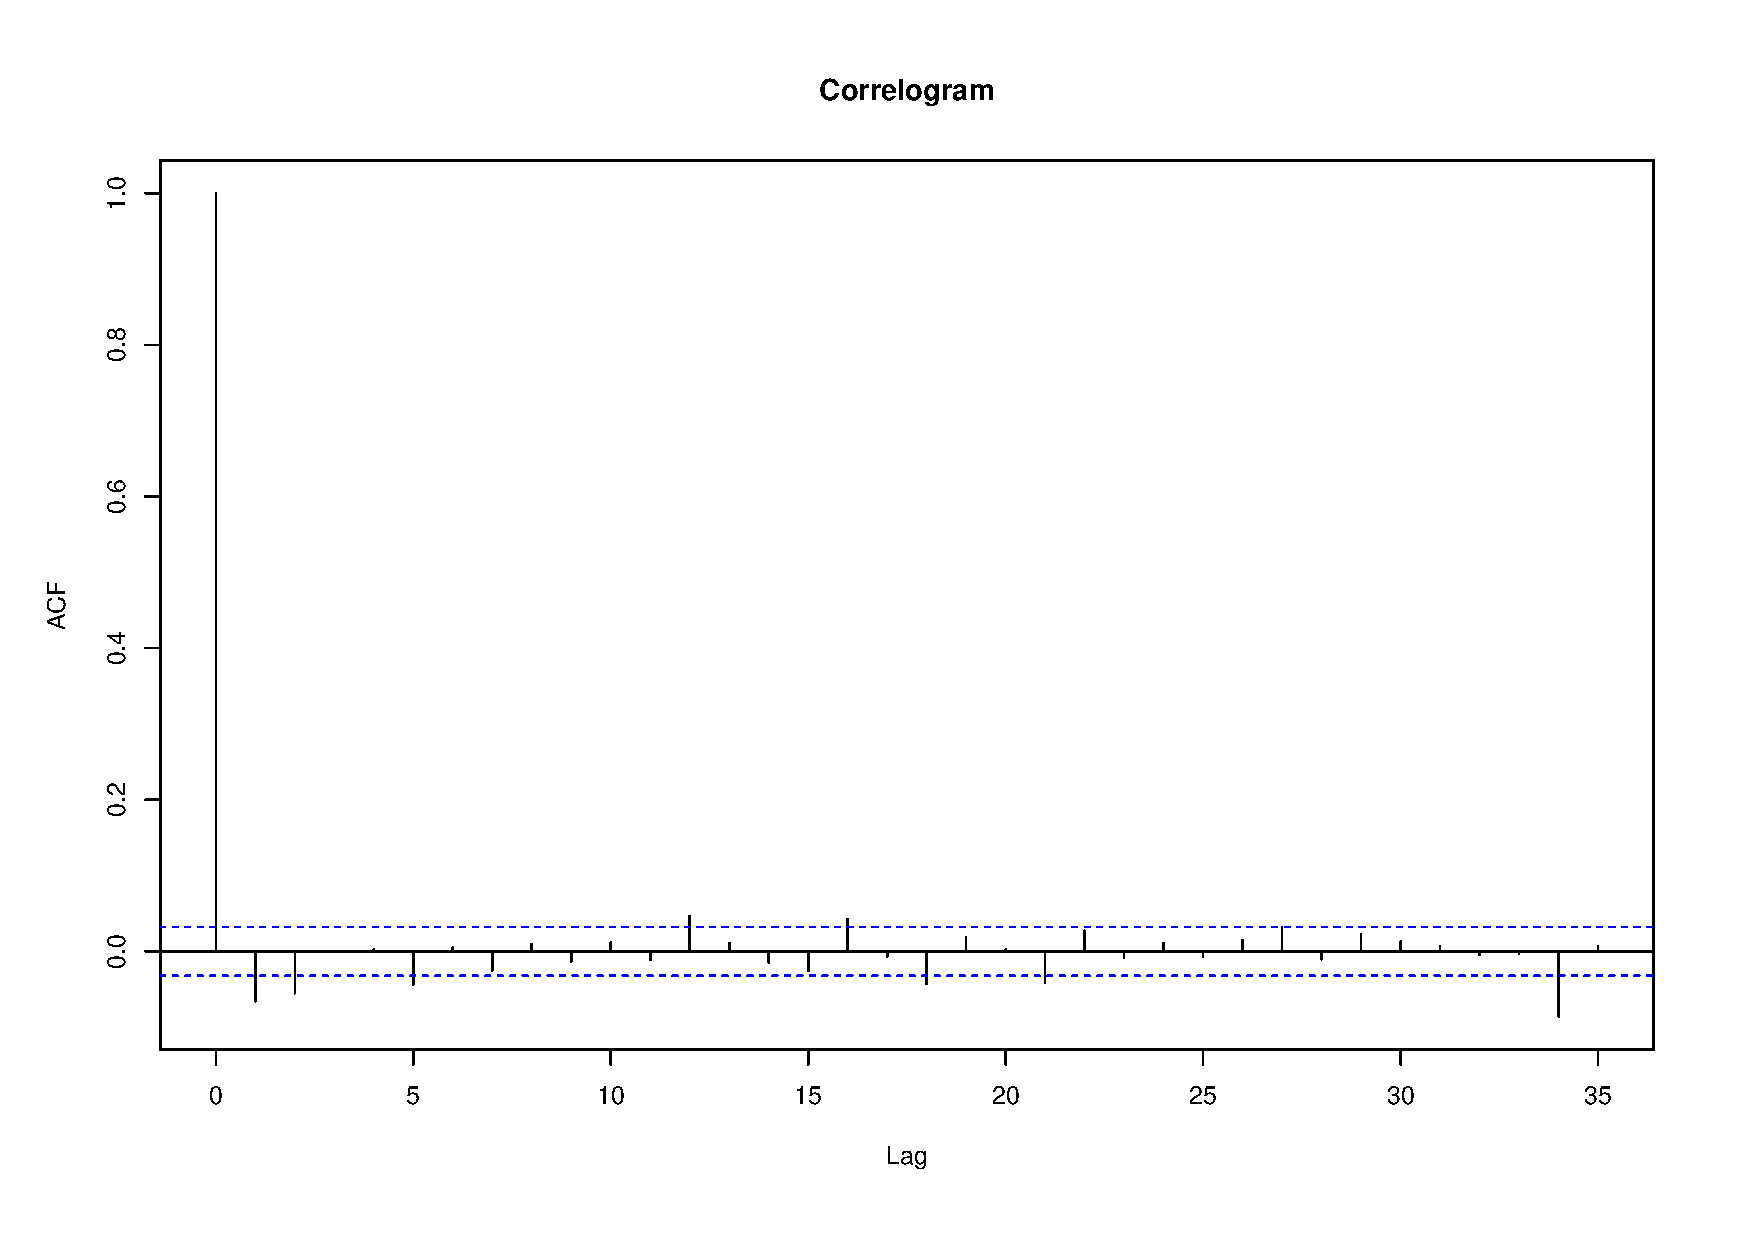
\includegraphics[scale=0.5]{plots/spy_returns_acf.pdf}
 % spy_returns_dist.pdf: 504x504 pixel, 72dpi, 17.78x17.78 cm, bb=0 0 504 504
 \caption{SPY returns ACF}
 \label{fig:returnacf}
\end{figure}

 \item[Returns distribution] The returns distribution has fat tails, i.e. the number of extreme events (either positive or negative) returns is larger than what is hypothesized by common data generation process (generally normal distribution assumption). In the markets, fat tails are an undesirable feature because of the additional risk they imply.
 In the figure \ref{fig:returndist} is shown the SPY returns distribution based on daily dates from the period 1st July 1998 to 4th April 2013. The distribution was compared against the normal distribution which clearly doesn't fit the data.  
 
 
 \begin{figure}[h]
 \centering
 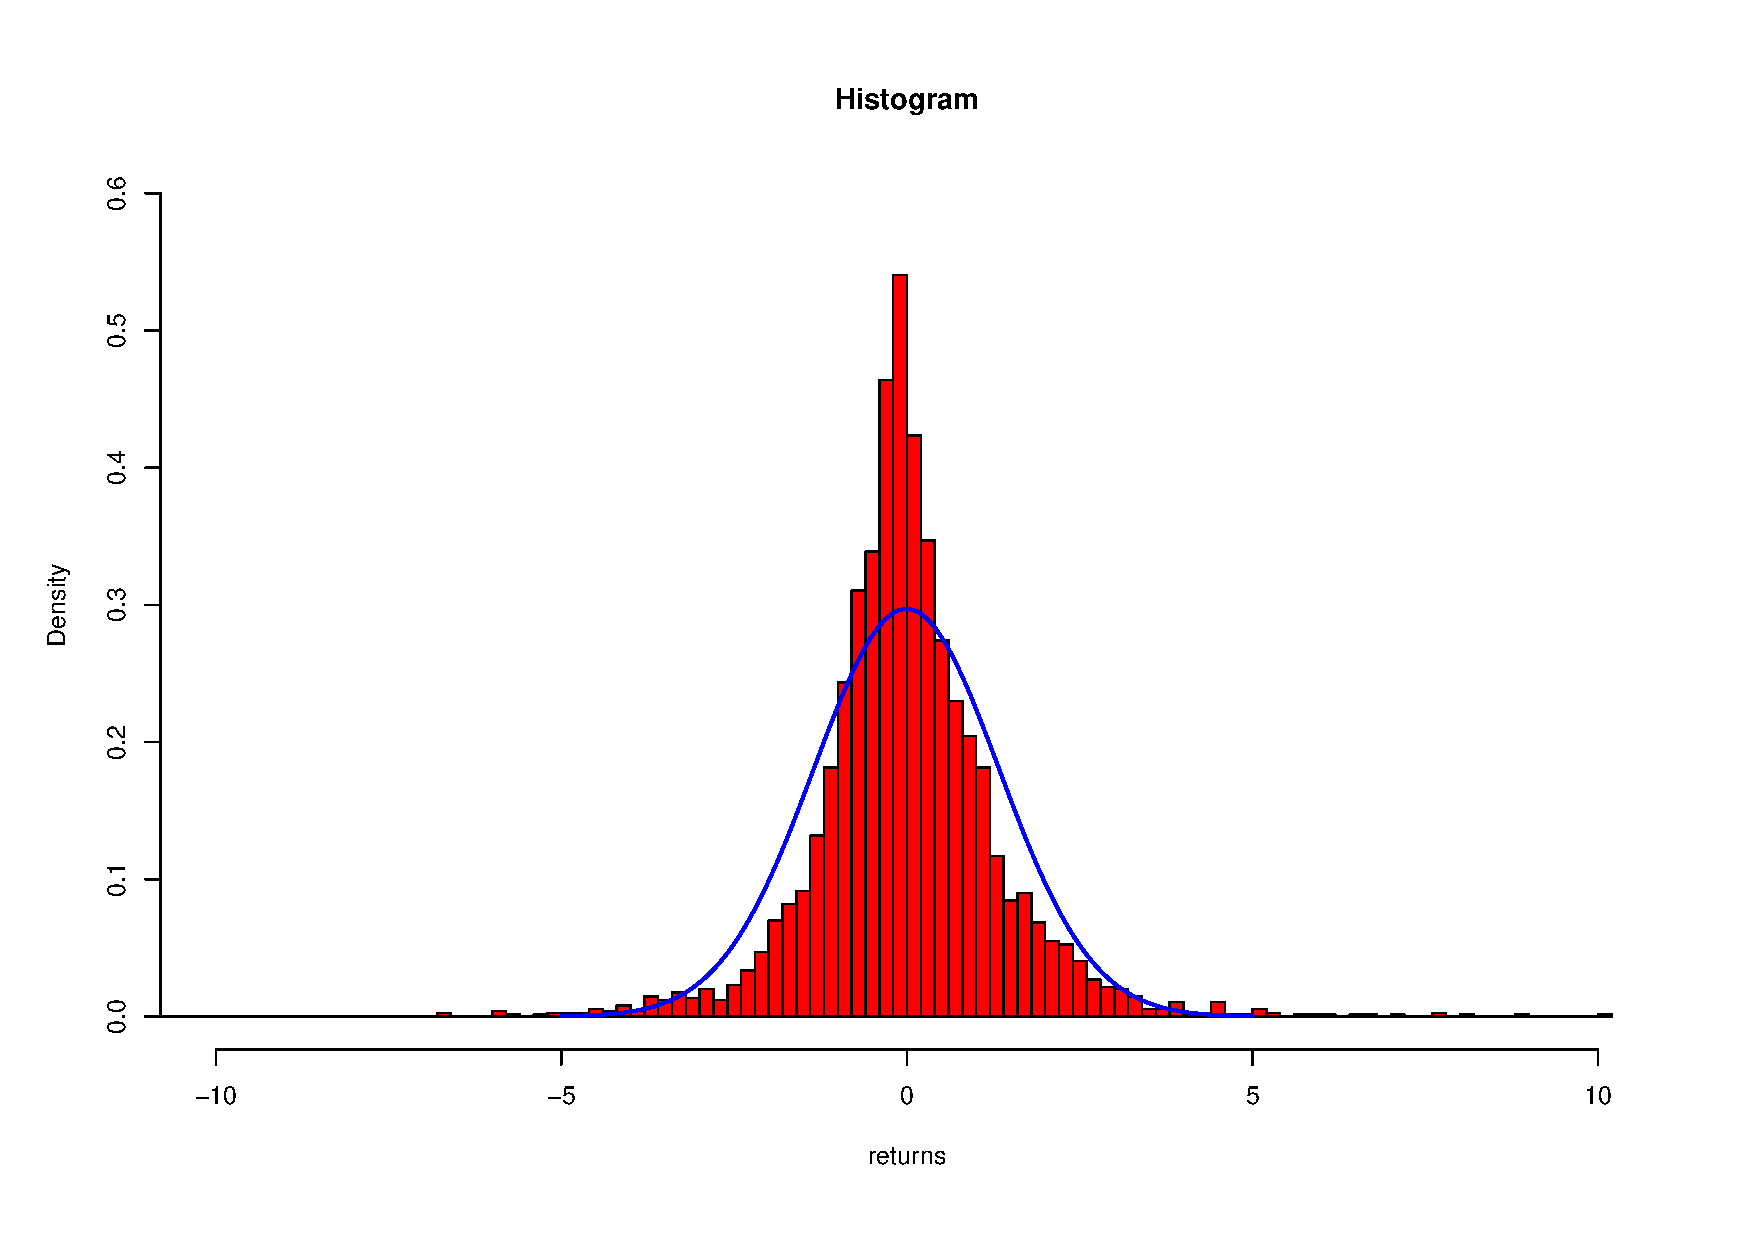
\includegraphics[scale=0.5]{plots/spy_returns_dist.pdf}
 % spy_returns_dist.pdf: 504x504 pixel, 72dpi, 17.78x17.78 cm, bb=0 0 504 504
 \caption{SPY returns distribution}
 \label{fig:returndist}
\end{figure}

 \item[Volume] refers to the level of trading activity in a market.
 \item[Calendar effects] days of week, weekend, holidays.
 \item[Intraday effects] time of the day.
 \item[Overnight effects]
\end{description}
